\documentclass{cmspaper}
\usepackage{graphicx}
\usepackage{subfigure}
\usepackage{amsmath}
\usepackage{amssymb}
\usepackage[pdfborder=0 0 0,
            colorlinks,
            urlcolor = blue,
            linkcolor = black,
            citecolor = black,
            menucolor = black,]
           {hyperref}
%% \usepackage[colorlinks]{hyperref}
%% \usepackage{url}
\usepackage[toc,page]{appendix}
\renewcommand{\appendixname}{Appendix}
%% \renewcommand{\appendixtocname}{List of appendices}

\newcommand{\CLs}{\ensuremath{CL_\mathrm{s}}}
\newcommand{\CLb}{\ensuremath{CL_\mathrm{b}}}
\newcommand{\CLsb}{\ensuremath{CL_\mathrm{s+b}}}

\newcommand{\GeV}{\ensuremath{\mathrm{Ge\kern -0.1em V}}}
\newcommand{\TeV}{\ensuremath{\mathrm{Te\kern -0.1em V}}}
\newcommand{\TeVcc}{\ensuremath{\,\mathrm{Te\kern -0.1em V\!/c}^2}}
\newcommand{\GeVcc}{\ensuremath{\,\mathrm{Ge\kern -0.1em V\!/c}^2}}
\newcommand{\MeVcc}{\ensuremath{\,\mathrm{Me\kern -0.1em V\!/c}^2}}
\newcommand{\GeVc}{\ensuremath{\mathrm{Ge\kern -0.1em V}\!/c}}
\newcommand{\nanob}{\mbox{{\rm ~nb}~}}
\newcommand{\fb}{\ensuremath{\mathrm{fb}}}
\newcommand{\pb}{\ensuremath{\mathrm{pb}}}
\newcommand{\ifb}{\ensuremath{\mathrm{fb^{-1}}}}
\newcommand{\ipb}{\ensuremath{\mathrm{pb^{-1}}}}
\newcommand{\grad}{\ensuremath{^{\circ}}}
%
% Special user made math symbols
%
\newcommand{\lsim}{\raisebox{-1.5mm}{$\:\stackrel{\textstyle{<}}{\textstyle{\sim}}\:$}}
\newcommand{\gsim}{\raisebox{-1.5mm}{$\:\stackrel{\textstyle{>}}{\textstyle{\sim}}\:$}}

% particles

\newcommand{\pipm}{\ensuremath{\pi^{\pm}}}
\newcommand{\pizero}{\ensuremath{\pi^{0}}}
\newcommand{\Hi}{\ensuremath{\mathrm{H}}}
\newcommand{\W}{\ensuremath{\mathrm{W}}}
\newcommand{\Wjets}{\ensuremath{\mathrm{W+jets}}}
\newcommand{\Zjets}{\ensuremath{\mathrm{Z+jets}}}
\newcommand{\Wt}{\ensuremath{\mathrm{Wt}}}
\newcommand{\Wstar}{\ensuremath{\mathrm{W}^{*}}}
\newcommand{\Wparenthesisstar}{\ensuremath{\mathrm{W}^{(*)}}}
\newcommand{\WW}{\ensuremath{\W^+\W^-}}
\newcommand{\Z}{\ensuremath{\mathrm{Z}}}
\newcommand{\Zstar}{\ensuremath{\mathrm{Z}^{*}}}
\newcommand{\Astar}{\ensuremath{\mathrm{\gamma}^{*}}}
\newcommand{\ZZ}{\ensuremath{\Z\Z}}
\newcommand{\WZ}{\ensuremath{\W\Z}}
\newcommand{\Wgstar}{\ensuremath{\W\Astar}}
\newcommand{\E}{\ensuremath{\mathrm{e}}}
\newcommand{\Ep}{\ensuremath{\mathrm{e}^{+}}}
\newcommand{\Em}{\ensuremath{\mathrm{e}^{-}}}
\newcommand{\Epm}{\ensuremath{\mathrm{e}^{\pm}}}
\newcommand{\Emp}{\ensuremath{\mathrm{e}^{\mp}}}
\newcommand{\M}{\ensuremath{\mu}}
\newcommand{\Mp}{\ensuremath{\mu^{+}}}
\newcommand{\Mm}{\ensuremath{\mu^{-}}}
\newcommand{\Mpm}{\ensuremath{\mu^{\pm}}}
\newcommand{\Mmp}{\ensuremath{\mu^{\mp}}}
\newcommand{\Tau}{\ensuremath{\tau}}
\newcommand{\Nu}{\ensuremath{\nu}}
\newcommand{\Nubar}{\ensuremath{\bar{\nu}}}
\newcommand{\Lep}{\ensuremath{\ell}}
\newcommand{\Lepp}{\ensuremath{\ell^{+}}}
\newcommand{\Lepm}{\ensuremath{\ell^{-}}}
\newcommand{\Lprime}{\ensuremath{\Lep^{\prime}}}
\newcommand{\Prot}{\ensuremath{\mathrm{p}}}
\newcommand{\Pbar}{\ensuremath{\bar{\mathrm{p}}}}
\newcommand{\PP}{\Prot\Prot}
\newcommand{\PPbar}{\Prot\Pbar}
\newcommand{\ttbar}{\ensuremath{\mathrm{t}\bar{\mathrm{t}}}}
\newcommand{\qq}{\ensuremath{\mathrm{q}\mathrm{q}}}
%\newcommand{\bbbar}{\ensuremath{\mathrm{b}\bar{\mathrm{b}}}}
\newcommand{\Wtb}{\ensuremath{\W\mathrm{t}\mathrm{b}}}
\newcommand{\Top}{\ensuremath{\mathrm{t}}}
\newcommand{\Bot}{\ensuremath{\mathrm{b}}}
\newcommand{\Atop}{\ensuremath{\bar{\mathrm{t}}}}
\newcommand{\Abot}{\ensuremath{\bar{\mathrm{b}}}}
% arrow
\newcommand{\To}{\ensuremath{\rightarrow}}

% masses
\newcommand{\mHi}{\ensuremath{m_{\mathrm{H}}}}
\newcommand{\mW}{\ensuremath{m_{\mathrm{W}}}}
\newcommand{\mZ}{\ensuremath{m_{\mathrm{Z}}}}
\newcommand{\mll}{\ensuremath{m_{\Lep\Lep}}}
\newcommand{\mt}{\ensuremath{m_{\mathrm{T}}}}

% kinematics
\newcommand{\pt}{\ensuremath{p_\mathrm{T}}}
\newcommand{\ptveto}{\ensuremath{\pt^\mathrm{veto}}}
\newcommand{\ptl}{\ensuremath{p_\perp^{\Lep}}}
\newcommand{\ptlmax}{\ensuremath{p_{\mathrm{T}}^{\Lep,\mathrm{max}}}}
\newcommand{\ptlmin}{\ensuremath{p_{\mathrm{T}}^{\Lep,\mathrm{min}}}}
\newcommand{\met}{\ensuremath{\Et^{\mathrm{miss}}}}
\newcommand{\delphill}{\ensuremath{\Delta\phi_{\Lep\Lep}}}
\newcommand{\deletall}{\ensuremath{\Delta\eta_{\Lep\Lep}}}
\newcommand{\delphimetl}{\ensuremath{\Delta\phi_{\met\Lep}}}
\newcommand{\Et}{\ensuremath{E_\mathrm{T}}}
\newcommand{\delR}{\ensuremath{\Delta R}}
\newcommand{\Eta}{\ensuremath{\eta}}

%efficiencies
\newcommand{\effsig}{\ensuremath{\varepsilon_{\mathrm{bkg}}^{\mathrm{S}}}}
\newcommand{\effnorm}{\ensuremath{\varepsilon_{\mathrm{bkg}}^{\mathrm{N}}}}
\newcommand{\Nsig}{\ensuremath{N_{\mathrm{bkg}}^{\mathrm{S}}}}
\newcommand{\Nnorm}{\ensuremath{N_{\mathrm{bkg}}^{\mathrm{N}}}}

% processes
\newcommand{\dyee}{\ensuremath{Z/\gamma^*\to ee}}
\newcommand{\dymm}{\ensuremath{Z/\gamma^*\to\mu\mu}}
\newcommand{\dytt}{\ensuremath{Z/\gamma^*\to\tau\tau}}
\newcommand{\dyll}{\ensuremath{Z/\gamma^*\to\ell\ell}}
\newcommand{\dy}{\ensuremath{Z/\gamma^*}}
\newcommand{\zee}{\ensuremath{Z\to ee}}
\newcommand{\zmm}{\ensuremath{Z\to\mu\mu}}
\newcommand{\ztt}{\ensuremath{Z\to\tau\tau}}
%\newcommand{\ttbar}{\ensuremath{t\bar{t}}}
\newcommand{\ppww}{\ensuremath{pp \to W^+W^-}}
\newcommand{\wwll}{\ensuremath{WW\to \ell^+\ell^-}}
\newcommand{\wwlnln}{\ensuremath{W^+W^-\to \ell^+\nu \ell^-\bar{\nu}}}
\newcommand{\ww}{\ensuremath{WW}}
\newcommand{\wwpm}{\ensuremath{W^+W^-}}
\newcommand{\hww}{\ensuremath{H\to W^+W^-}}
\newcommand{\wz}{\ensuremath{WZ}}
\newcommand{\zz}{\ensuremath{ZZ}}
\newcommand{\wgamma}{\ensuremath{W\gamma}}
\newcommand{\wjets}{\ensuremath{W+}jets} 
\newcommand{\tw}{\ensuremath{tW}} 
\newcommand{\singletopt}{\ensuremath{t} ($t$-chan)} 
\newcommand{\singletops}{\ensuremath{t} ($s$-chan)} 
\newcommand{\zx}{\ensuremath{\mathrm{DY/WZ/ZZ}}}
\newcommand{\zv}{\ensuremath{\mathrm{WZ/ZZ}}}
\newcommand{\z}{\ensuremath{\mathrm{Z}}}
\newcommand{\routin}{\ensuremath{R_{out/in}}}

%other 
\def\fixme{({\bf FixMe})}
\newcommand{\ee}{\ensuremath{ee}}
\newcommand{\emu}{\ensuremath{e\mu}}
\def\mm{\ensuremath{\mu\mu}}

% integrated luminosity
\newcommand{\intlumiSevenTeV}{4.92~\ifb}
\newcommand{\intlumiEightTeV}{1.62~\ifb}

%%%%%%%%%%%
%
\newcounter{myfootertablecounter}

\newcommand\myfootnotemark{%
  %\refstepcounter{footnote}%
  \addtocounter{footnote}{1}%
  \footnotemark[\thefootnote]%
}%

\newcommand\myfootnotetext[1]{%
  \addtocounter{myfootertablecounter}{1}
  \footnotetext[\value{myfootertablecounter}]{#1}
}

% from now on, myfootnote has to be used rather than footnote to
% adapt the myfootercounter
\newcommand\myfootnote[1]{%
  \addtocounter{myfootertablecounter}{1}
  \footnote{#1}
}%


% useful definitions

% processes
\def\dyee {\ensuremath{Z/\gamma^*\to ee}}
\def\dymm {\ensuremath{Z/\gamma^*\to\mu\mu}}
\def\dytt {\ensuremath{Z/\gamma^*\to\tau\tau}}
\def\zee {\ensuremath{Z\to ee}}
\def\zmm {\ensuremath{Z\to\mu\mu}}
\def\ztt {\ensuremath{Z\to\tau\tau}}
\def\ttbar {\ensuremath{t\bar{t}}}
\def\wwll {\ensuremath{WW\to l^+l^-}}
\def\wwlulu{\ensuremath{WW\to l^+\nu l^-\bar{\nu}}}
\def\ww {\ensuremath{WW}}
\def\hww {\ensuremath{H\to WW}}
\def\wz{\ensuremath{WZ}}
\def\zz{\ensuremath{ZZ}}
\def\wgamma{\ensuremath{W\gamma}}
\def\wjets{\ensuremath{W+}jets} 
\def\tw{\ensuremath{tW}} 
\def\singletopt{\ensuremath{t} ($t$-chan)} 
\def\singletops{\ensuremath{t} ($s$-chan)} 
\def\all{all}
\def\ee{\ensuremath{ee}}
\def\emu{\ensuremath{e\mu}}
\def\mm{\ensuremath{\mu\mu}}

%units
\newcommand{\TeV}{\ensuremath{\mathrm{Te\kern -0.1em V}}}
\newcommand{\GeV}{\ensuremath{\mathrm{Ge\kern -0.1em V}}}

%others
\def\pt{\ensuremath{p_T}}
\def\ipb{pb\ensuremath{^{-1}}}
\def\ifb{fb\ensuremath{^{-1}}}
\def\et{\ensuremath{E_T}}
\def\met{\ensuremath{E\!\!\!\!/_T}}
\def\fBrem{\ensuremath{f_{\rm brem}}}
\def\pin{\ensuremath{p_{\rm in}}}
\def\pout{\ensuremath{p_{\rm out}}}


\setcounter{topnumber}{1}
\setcounter{bottomnumber}{1}

\begin{document}
\begin{titlepage}

  \analysisnote{2012/XXX}

  \date{\today}

  \title{Estimating the Drell-Yan Contribution to a Dilepton + MET Selection using Photon+Jets Events
  for HWW Analysis}
  
  \begin{Authlist}
%
L.~Bauerdick, K.~Burkett, I.~Fisk, Y.~Gao, O.~Gutsche, B.~Hooberman, S.~Jindariani, S.~Tkaczyk, V. Martinez Outschoorn, 
\Instfoot{fnal}{Fermilab National Accelerator Laboratory, Batavia, USA}
%
G.~Bauer, J.~Bendavid, E.~Butz, M.~Chan, V.~Dutta, G.~G\'omez-Ceballos, M.~Goncharov, K.~Hahn, P.~Harris, M.~Klute, S.~Nahn, C.~Paus, D.~Ralph, F.~Stoeckli, K.~Sumorok, K.~Sung, R.~Wolf, S.~Xie, M.~Yang, M.~Zanetti
\Instfoot{mit}{Laboratory for Nuclear Science, Massachusetts Institute of Technology, Cambridge, USA}
%
D.~Barge, C.~Campagnari, D.~Kovalskyi, V.~Krutelyov
\Instfoot{ucsb}{University of California, Santa Barbara, Santa Barbara, USA}
%
W.~Andrews, G.~Cerati, D.~Evans, F.~Golf, I.~MacNeill, S.~Padhi, Y.~Tu, F.~W\"urthwein, A.~Yagil, J.~Yoo
\Instfoot{ucsd}{University of California, San Diego, San Diego, USA}
%
I.~Kravchenko
\Instfoot{unl}{University of Nebraska-Lincoln, USA}

\end{Authlist}


  \begin{abstract}
The selection of events containing dileptons + MET is important for both Standard Model measurements and searches for new physics. If both leptons have the same flavour, then a background may be introduced from the Drell-Yan process where the MET arises due to instrumental mis-measurement.  A data driven method to estimate this background by using a photon+jets control region is described in this note in the context of the Higgs boson search in the {$\mathrm{WW}\rightarrow\ell\nu\ell\nu$} channel.
   \end{abstract} 

\end{titlepage}
\tableofcontents
\listoftables
\listoffigures
\newpage 

\section{Introduction}
   \label{sec:introduction}
   Precision measurement of the gauge boson couplings is a well known
method to look for physics beyond the Standard Model. In the case of
the triple gauge boson couplings, new physics contributions can be
expressed in the form of an effective Lagrangian. The most general
form of such a Lagrangian has 14 complex couplings (7 for $WWZ$ and 7 for
$WW\gamma$). Assuming electromagnetic gauge invariance, and C and P
symmetry conservation that number is reduced to five:
$\Delta\kappa_Z$, $\Delta g^Z_1$, $\Delta\kappa_{\gamma}$, $\lambda_Z$
and $\lambda_{\gamma}$. Applying gauge constraints:
\begin{align}
  \Delta\kappa_Z &= \Delta g^Z_1- \Delta\kappa_{\gamma}\tan^2\theta_W \\
  \lambda_Z &= \lambda_{\gamma}
\end{align}
further reduces the number of independent couplings to three. In the
Standard Model all five couplings are zero. 
 
CMS performed a first measurement of the anomalous couplings with
35/pb of data at 7 TeV~\cite{blah}. The measurement was performed with
and without a form factor that helps to avoid unitarity violation by
introducing an effective cutoff scale where a coupling is switched
off.  In this study we have two orders of magnitude more data and
experimental constraints on the couplings are more stringent then the
unitarity constraint. Therefore all the anomalous couplings are
form-factor free.

This analysis is based on the $W^+W^-$ production cross-section
measurement in $\intlumi$ of $pp$ collision data at $\sqrt{s} = $
7~$\TeV$ (the full 2011 dataset) \cite{ref:WWXS2011}. 

measurement~\cite{ref:WWXS2011}. Here we just briefly summarize the event
selection showing mostly kinematic requirements that may affect the
leading lepton pt distribution, which is used as a main observable.

The kinematic observable used in this analysis is 
the transverse momentum (\pt) of the leading lepton,
shown in Figure \ref{fig:pas_pt1_incl} after all event selections
have been applied.

\begin{figure}[hb]
\subfigure[Linear scale]{\label{subfig:pas_pt1_incl}
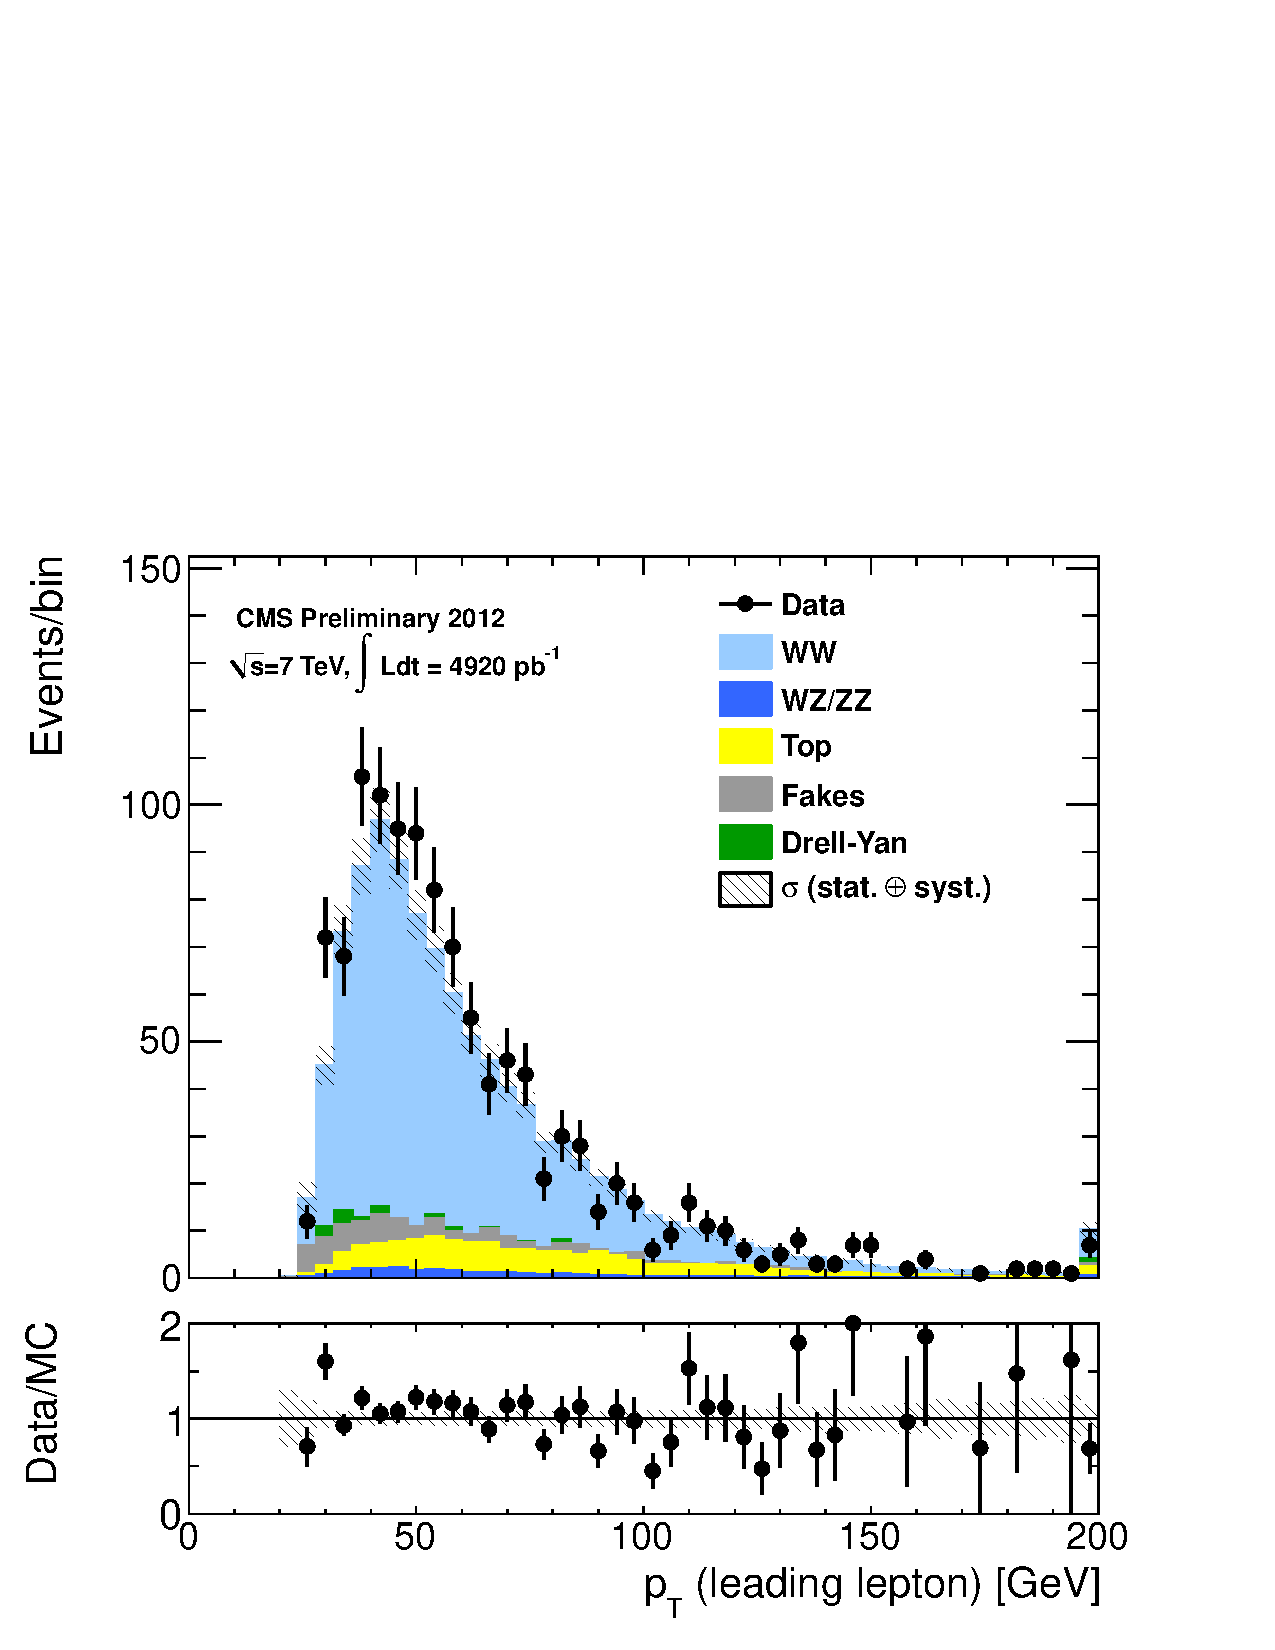
\includegraphics[width=.45\textwidth]{figures/pas_pt1_incl.pdf}}
\subfigure[Log scale]{\label{subfig:pas_pt1_incl_log}
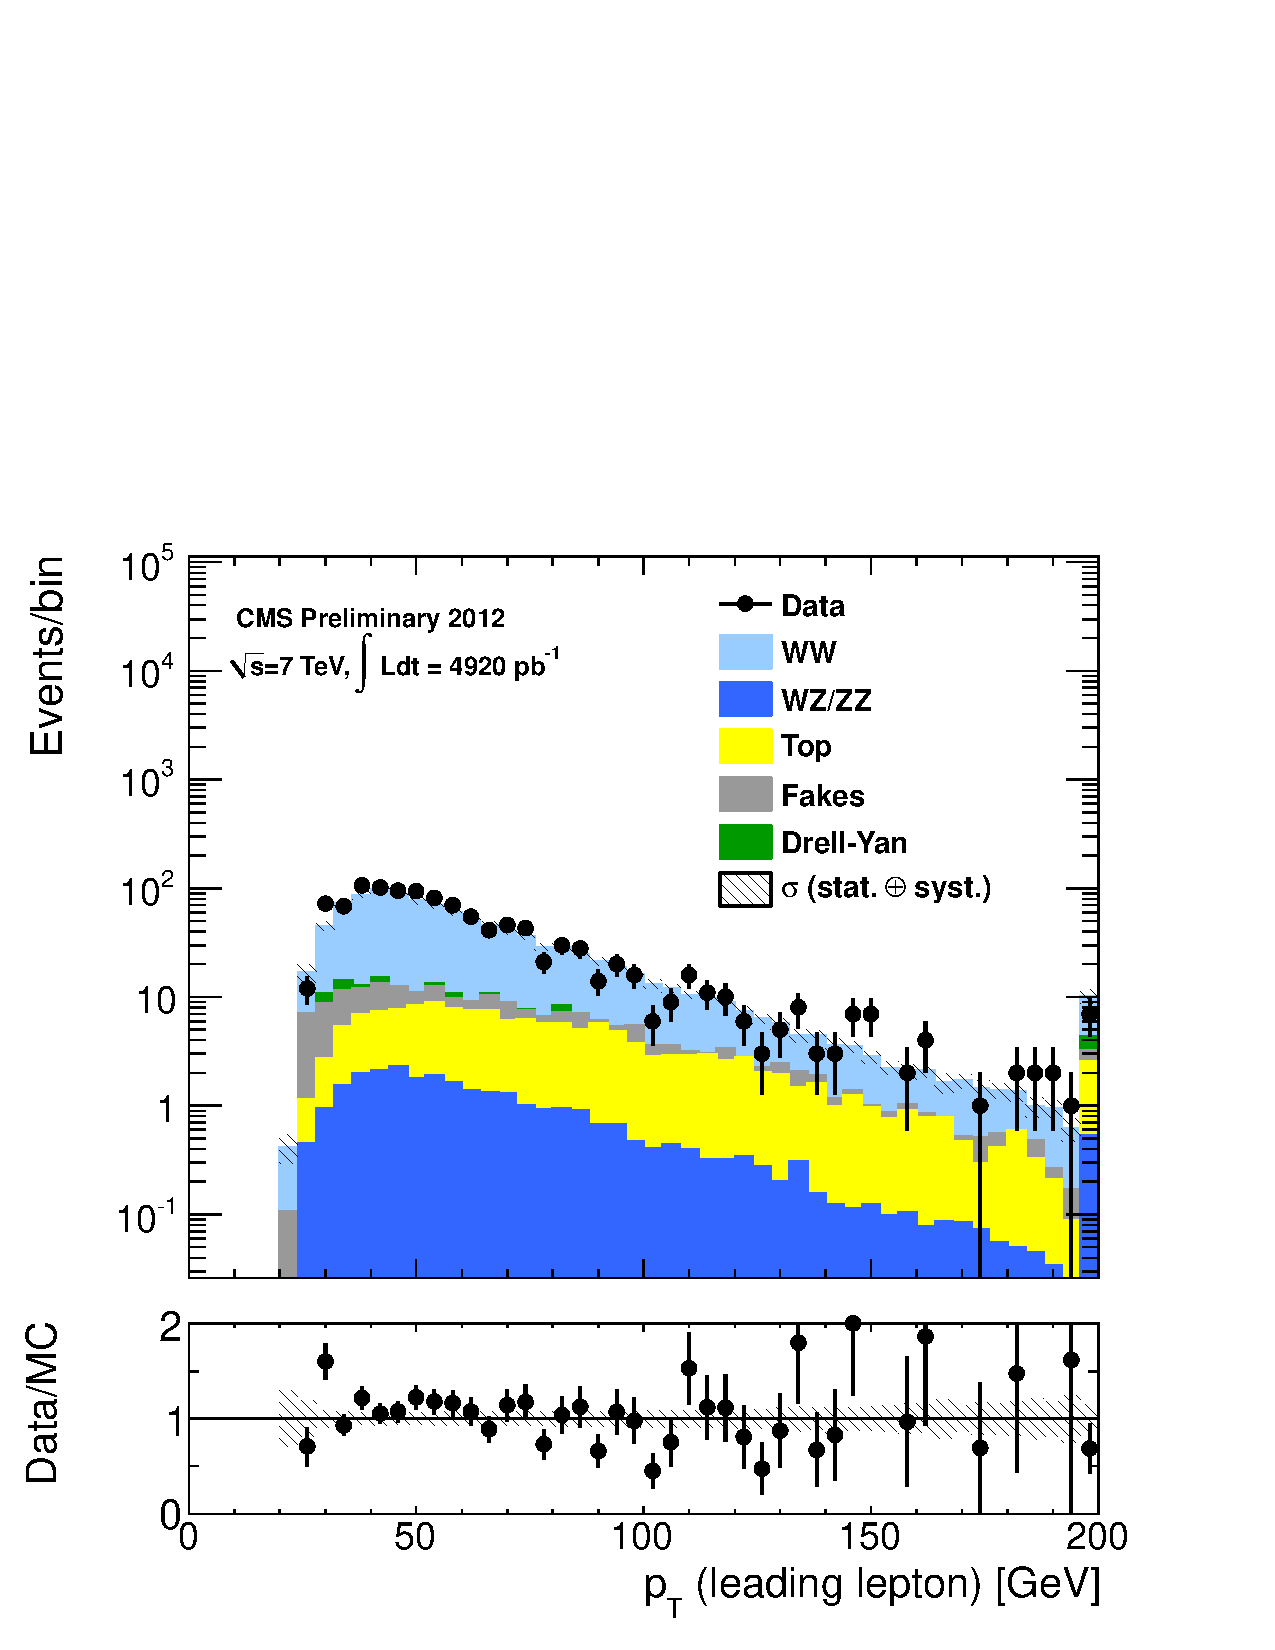
\includegraphics[width=.45\textwidth]{figures/pas_pt1_incl_log.pdf}}
\caption{Leading lepton \pt.}
\label{fig:pas_pt1_incl}
\end{figure}


\section{Samples and Selections}
  \label{sec:datasets}
  %UPDATEME%
The datasets used for this analysis are summarized in Tables.~\ref{tab:DatasetsData} 
and~\ref{tab:DatasetsMC} for data and Monte Carlo, respectively. The total integrated
luminosity is 49 $\pm$ 2 $\ipb$. We used just basic quality requirements, since an official good 
run list (JSON file) was not available. It will be used in future updates.
For Monte Carlo simulation we use madgraph when possible, 
but different generators such as Pythia and Powheg 
are also used. 
%For $gg \to \WW$ a dedicated generator is used. For \wz\ and \zz\
%processes we use Pythia, since MadGraph samples are mixed with $\WW$ in
%a single $VV$ sample, which is difficult to use properly.

%The choice of the Monte Carlo samples depends on the sample
%availability, but in general we tried to be consistent and use a
%single generator - MadGraph. In the case of Drell-Yan, MadGraph samples
%are not adequate to cover the full mass spectrum. The main sample has a 50 $\GeVcc$ 
%minimum dilepton mass requirement, while the other one, covering
%the low mass region, has an additional requirement on extra jet
%activity. 
%We use madgraph when possible, but different generators are used for some samples
%For $gg \to \WW$ a dedicated generator is used. For \wz\ and \zz\
%processes we use Pythia, since MadGraph samples are mixed with $\WW$ in
%a single $VV$ sample, which is difficult to use properly.

%UPDATEME%
\begin{table}[!ht]
\begin{center}
\begin{tabular}{|c|c|}
\hline
 Dataset Description                   &   Dataset Name   \\
\hline
\hline
\multicolumn{2}{|c|}{$H \to \WW$ Signal Selection Samples} \\
\hline
Run2011A MuEl PromptReco            &  /MuEG/Run2011A-PromptReco-v*/AOD   \\
Run2011A DiMuon PromptReco          &  /DoubleMu/Run2011A-PromptReco-v*/AOD   \\
Run2011A SingleMuon PromptReco      &  /SingleMu/Run2011A-PromptReco-v*/AOD   \\
Run2011A DiElectron PromptReco      &  /DoubleElectron/Run2011A-PromptReco-v*/AOD   \\
\hline
\hline
\multicolumn{2}{|c|}{Fake Rate Measurement Samples} \\
\hline
Run2010A Jet  PromptReco            & /Jet/Run2011A-PromptReco-v*/AOD	\\
Run2010B Photon PromptReco          & /Photon/Run2011A-PromptReco-v*/AOD \\
\hline
\end{tabular}
\caption{Summary of data datasets used.\label{tab:DatasetsData}}
\end{center}
\end{table}

\begin{table}[!ht]
\begin{center}
{\footnotesize
\begin{tabular}{|c|c|c|}
\hline
\multicolumn{3}{|c|}{With Pileup: Processed dataset name is always} \\
\multicolumn{3}{|c|}{/Spring11-PU\_S1\_START311\_V1G1-v*/AODSIM} \\
\hline
 Dataset Description                     &   Primary Dataset Name   & cross-section (pb)\\
\hline
qq $\rightarrow WW$                  	 &   /VVJetsTo4L\_TuneD6T\_7TeV-madgraph-tauola                        &  43.0  \\
gg $\rightarrow WW \to 2l 2\nu$          &   /GluGluToWWTo4L\_TuneZ2\_7TeV-gg2ww-pythia6                       &   0.153\\
$\ttbar$                              	 &   /TTJets\_TuneZ2\_7TeV-madgraph-tauola                             & 157.5 \\
$\singletops$                  	 	 &   /TToBLNu\_TuneZ2\_s-channel\_7TeV-madgraph                        &  1.4 \\
$\singletopt$                  	 	 &   /TToBLNu\_TuneZ2\_t-channel\_7TeV-madgraph                        &  20.9 \\
tW                                    	 &   /TToBLNu\_TuneZ2\_tW-channel\_7TeV-madgraph                       &  10.6 \\
Z[20-inf] $\rightarrow ee$	  	 &   /DYToEE\_M-20\_CT10\_TuneZ2\_7TeV-powheg-pythia                   &  1666.0 \\
Z[20-inf] $\rightarrow \mu\mu$        	 &   /DYToMuMu\_M-20\_CT10\_TuneZ2\_7TeV-powheg-pythia                 &  1666.0 \\	       
Z[20-inf] $\rightarrow \tau\tau$  	 &   /DYToTauTau\_M-20\_CT10\_TuneZ2\_7TeV-powheg-pythia-tauola        &  1666.0 \\
Z[10-20]  $\rightarrow ee$	  	 &   /DYToEE\_M-10To20\_CT10\_TuneZ2\_7TeV-powheg-pythia               &  3892.9 \\
Z[10-20]  $\rightarrow \mu\mu$    	 &   /DYToMuMu\_M-10To20\_CT10\_TuneZ2\_7TeV-powheg-pythia             &  3892.9 \\
Z[10-20]  $\rightarrow \tau\tau$  	 &   /DYToTauTau\_M-10To20\_CT10\_TuneZ2\_7TeV-powheg-pythia-tauola    &  3892.9 \\
W/Z+$\gamma$                       	 &   /PhotonVJets\_7TeV-madgraph                                       &  165.0 \\
W $\rightarrow$ $\ell\nu$           	 &   /WJetsToLNu\_TuneZ2\_7TeV-madgraph-tauola                         &  31314.0 \\
WZ                               	 &   /WZtoAnything\_TuneZ2\_7TeV-pythia6-tauola                        &  18.2 \\
ZZ                               	 &   /ZZtoAnything\_TuneZ2\_7TeV-pythia6-tauola                        &   5.9\\
$gg \to H \to WW \to 2\ell2\nu$          &   /GluGluToHToWWTo2L2Nu\_M-*\_7TeV-powheg-pythia6                   & vary \\
$gg \to H \to WW \to \ell\tau2\nu$       &   /GluGluToHToWWTo2L2Nu\_M-*\_7TeV-powheg-pythia6                   & vary \\
$gg \to H \to WW \to 2\tau2\nu$          &   /GluGluToHToWWTo2Tau2Nu\_M-*\_7TeV-powheg-pythia6                 & vary \\
$qqH,~H \to WW \to 2\ell2\nu$            &   /VBF\_HToWWTo2L2Nu\_M-*\_7TeV-powheg-pythia6                      & vary \\
$qqH,~ H \to WW \to \ell\tau2\nu$	 &   /VBF\_HToWWTo2Tau2Nu\_M-*\_7TeV-powheg-pythia6                    & vary \\
$qqH,~H \to WW \to 2\tau2\nu$	         &   /VBF\_HToWWToLNuTauNu\_M-*\_7TeV-powheg-pythia6                   & vary \\
$WH/ZH/\ttbar H,~H\to WW$                &   /WH\_ZH\_TTH\_HToWW\_M-*\_7TeV-pythia6                            & vary \\
\hline
\hline
\end{tabular}
}
\caption{Summary of Monte Carlo datasets used.\label{tab:DatasetsMC}. The cross sections for a SM Higgs boson
is taken from the LHC Higgs cross-section working group~\cite{LHCHiggsCrossSectionWorkingGroup:2011ti}}
\end{center}
\end{table}

Due to details in the implementation of the Powheg calculation, the
resulting Higgs $\pt$ spectrum for $gg \to H$ has a much harder
spectrum compared with the most precise spectrum calculated to NNLO
with resummation to NNLL order, as illustrated in
Figure~\ref{fig:h160ww_pthiggs}(a). Therefore, the proper procedure is
to apply an event-by-event rewighting to the Powheg simulated
events. For the time being we correct the $gg \to H \to \WW$ jet bin
efficiency computed from the Powheg Monte Carlo sample, by a scale
factor which is approximately identical for all Higgs masses. The
scale factors applied to each jet bin in the Powheg simulation are
shown in Figure~\ref{fig:h160ww_pthiggs}(b). The jet definition is 
consitent with the one used in the analysis.

\begin{figure}[!htbp]
\begin{center}
   \subfigure[]{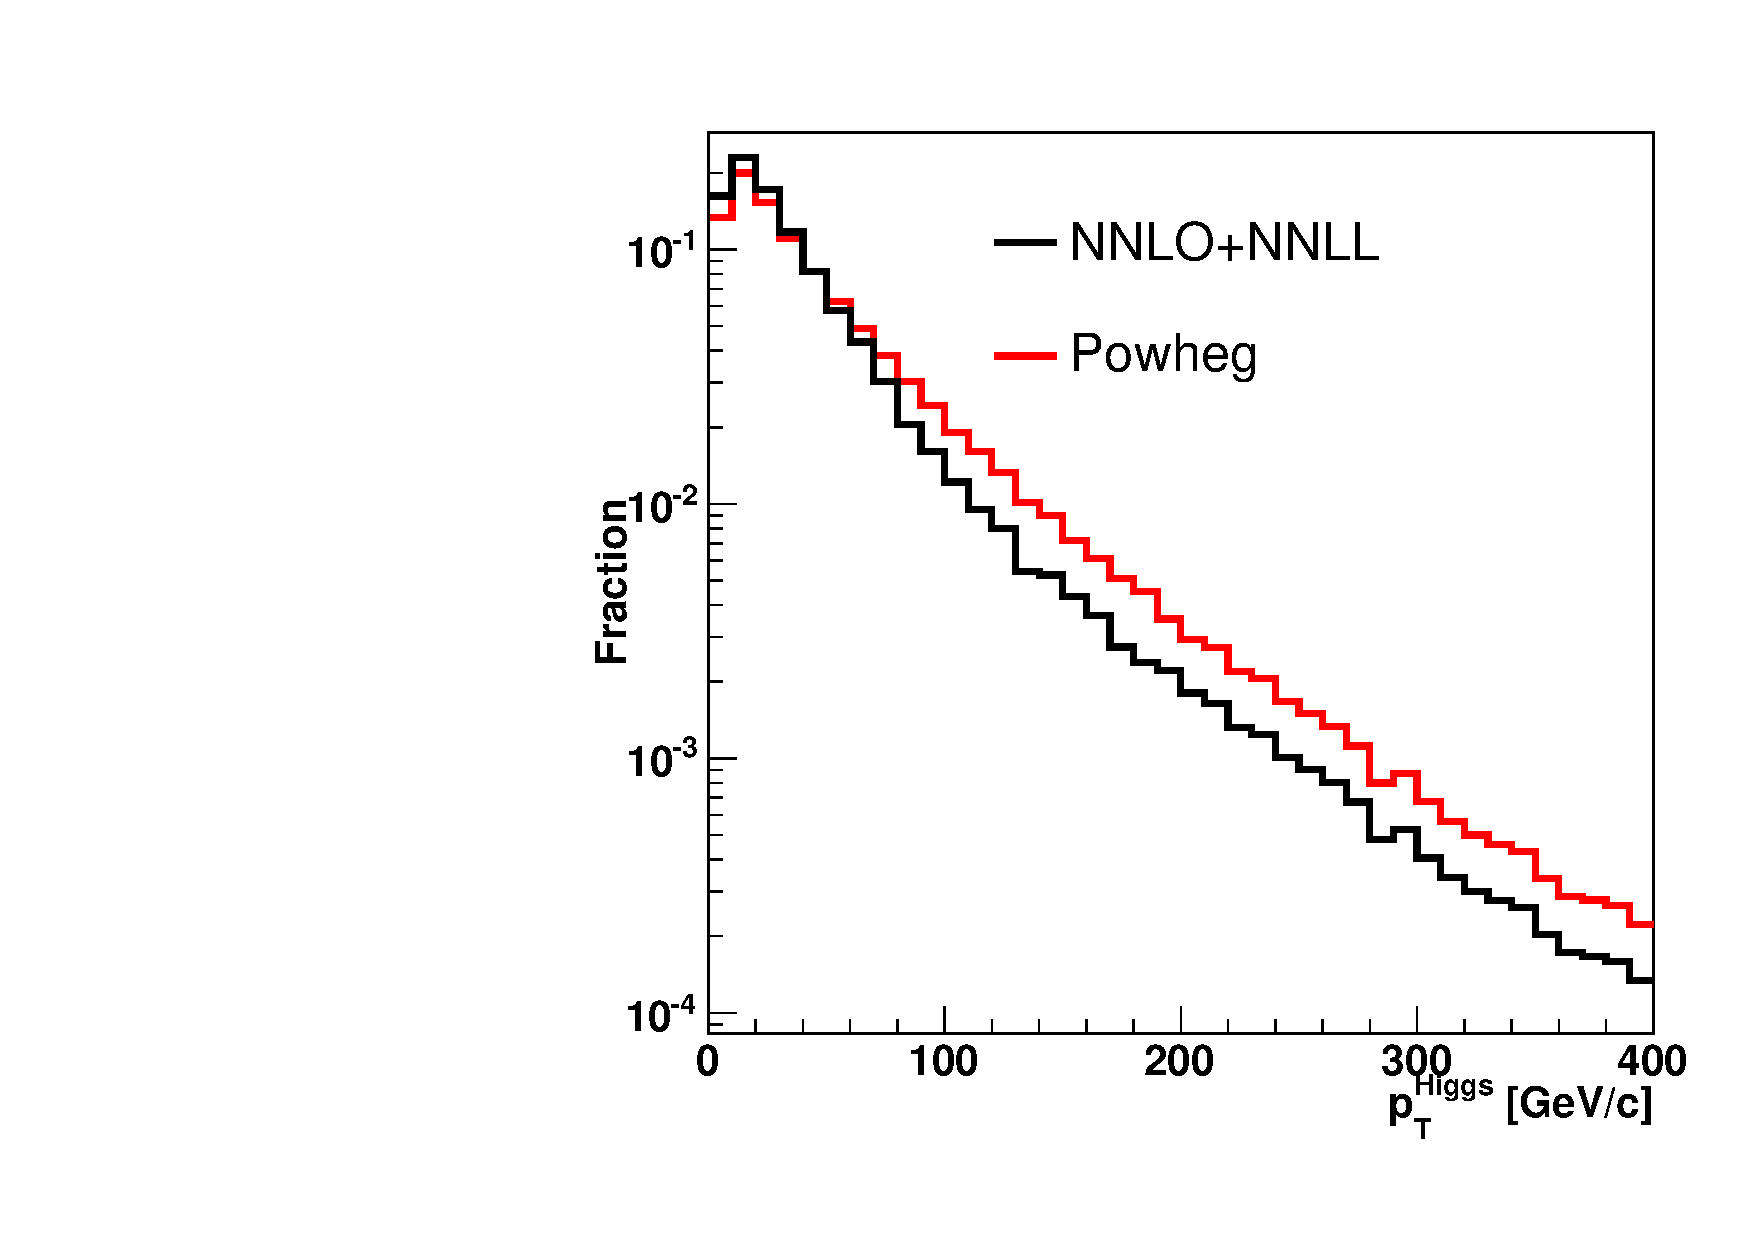
\includegraphics[width=0.49\textwidth]{figures/h160ww_pthiggs.pdf}}
   \subfigure[]{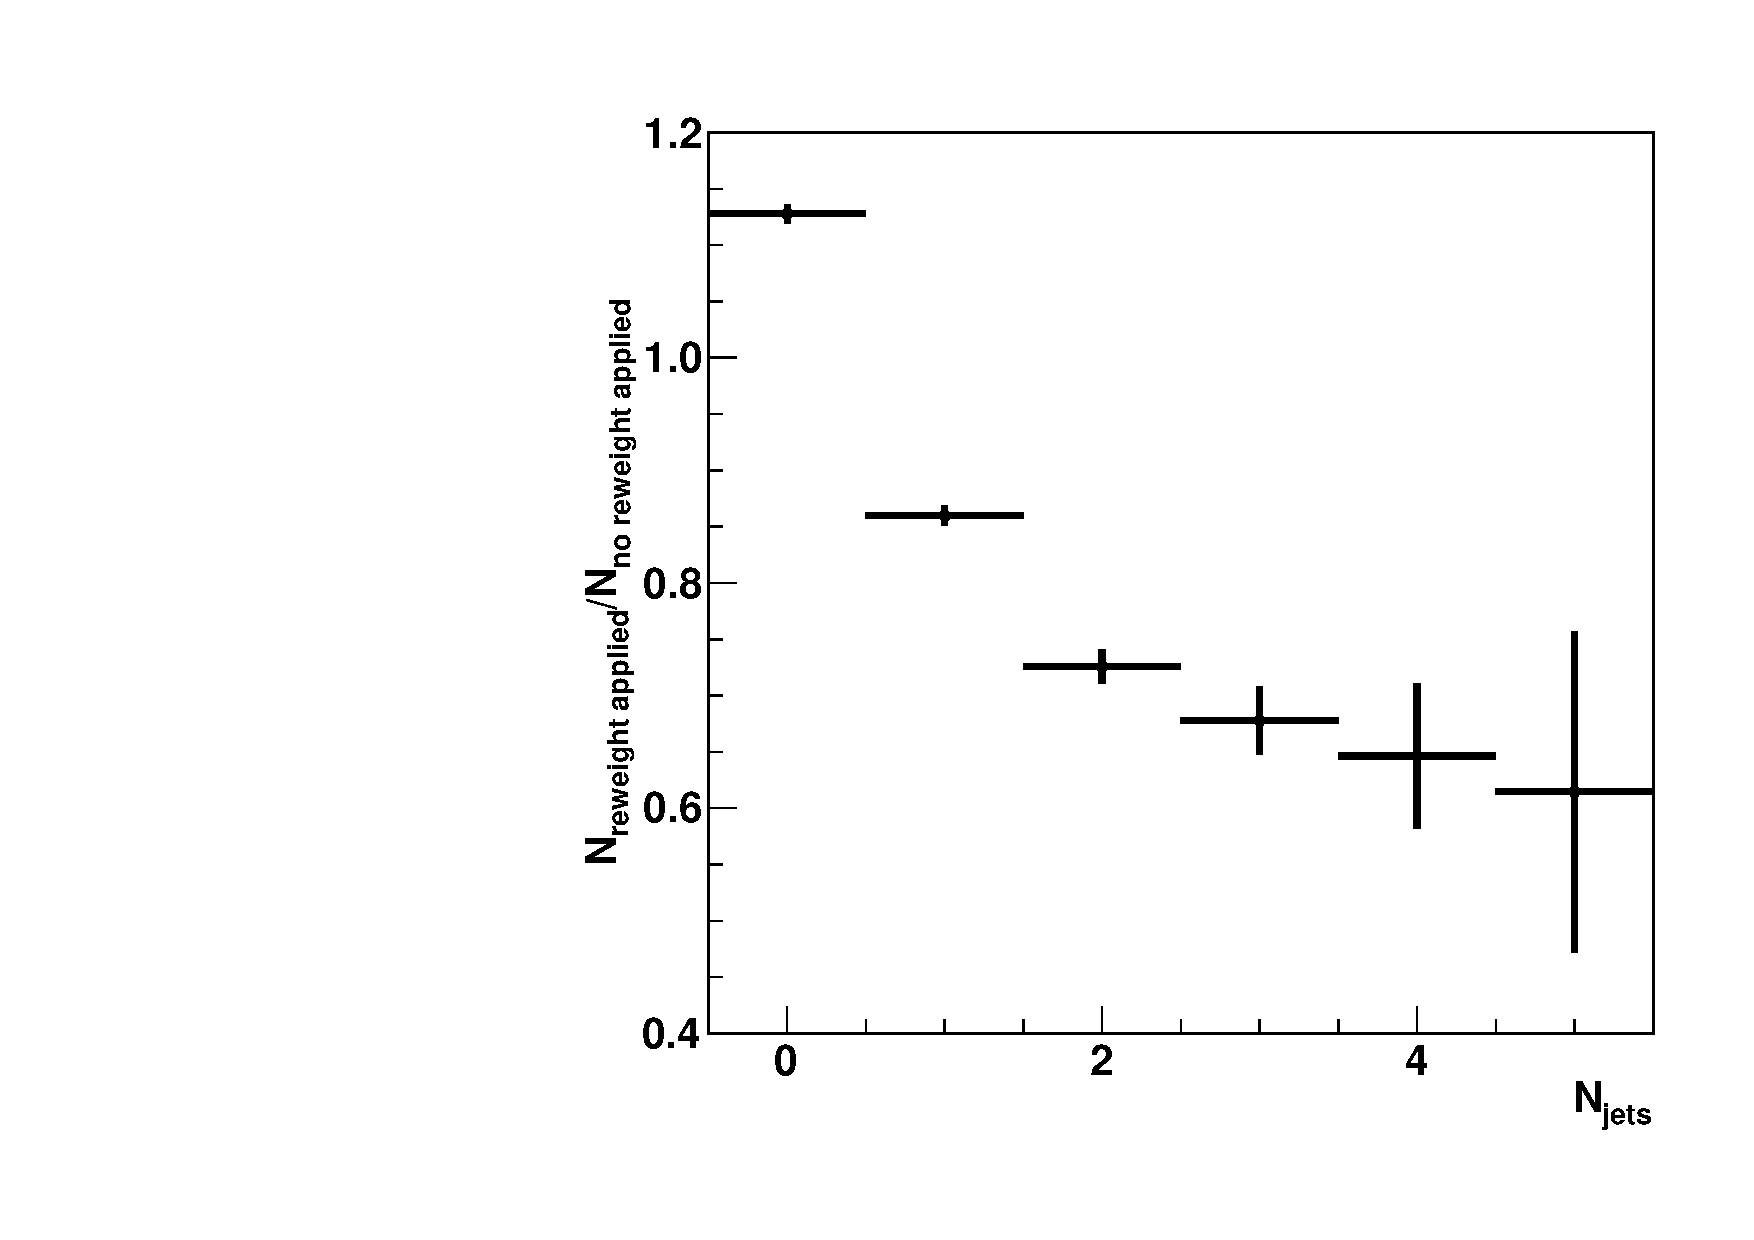
\includegraphics[width=0.49\textwidth]{figures/h160ww_njets_kfactor_ratio.pdf}} 
\caption{(a) Higgs transverse momentum spectrum as predicted by Powheg and the NNLO+NNLL calculation; (b) 
scale factors applied to each jet bin in the Powheg simulation.}
\label{fig:h160ww_pthiggs}
\end{center}
\end{figure}

\section{The \zm~ Method}
   \label{sec:method}
   In order to fit for anomalous couplings we used a maximum likelihood fit in
the RooFit framework. Differences between the Standard Model
and anomalous couplings are established in the leading lepton
\pt\ distribution and the overall \ww\ event yield. The combined PDF for the
leading lepton \pt\ distribution is:
\begin{equation}
  P(\pt) = \frac{N^\mathrm{exp}_\mathrm{sig}}{N^\mathrm{exp}}P_\mathrm{sig}(\pt) + 
  \frac{N^\mathrm{exp}_\mathrm{bkg}}{N^\mathrm{exp}}P_\mathrm{bkg}(\pt) 
\end{equation}
where $P_\mathrm{sig}$ and $P_\mathrm{bkg}$ are signal and background PDFs of the
leading lepton \pt{}, $N^\mathrm{exp}_\mathrm{sig}$ and $N^\mathrm{exp}_\mathrm{bkg}$ are the expected
number of signal and background events and
$N^\mathrm{exp}=N^\mathrm{exp}_\mathrm{sig}+N^\mathrm{exp}_\mathrm{bkg}$.

The Likelihood is defined as a product of Poisson PDFs for the observed
number of events and the combined PDF for each event:
\begin{equation}
  L = e^{-N^\mathrm{exp}}(N^\mathrm{exp})^{N^\mathrm{obs}}\displaystyle\prod_{i=1}^{N^\mathrm{obs}}P(\pt)
\end{equation}

To account for statistical and systematic uncertainties in the
luminosity, cross-section and background estimation we assume
Gaussian distributions for the uncertainties and add corresponding
constraints to the Likelihood.

The signal PDF allows for parameterization of the leading lepton \pt\
PDF and the cross-section as functions of the anomalous
couplings. Since the effective Lagrangian is linear in the couplings
we can parametrize the leading lepton differential cross-section with
a 2D or 3D parabola ~\cite{ref:atgc_method}. In the fit the expected
number of signal events is taken from that parameterization. The
expected background yield is taken from the background estimation of
the \ww\ analysis~\cite{ref:wwnote}. Table~\ref{tab:xsections} shows
the reference points and the corresponding cross-sections used in the
model.

\begin{table}[!ht]
  \begin{center}
  \begin{tabular} {|c c c|c c|c|}
\hline
  $\lambda_Z$ & $\Delta g^Z_1$ & $\Delta\kappa_{\gamma}$ & $\Delta\kappa_Z$ & $\lambda_{\gamma}$ & $\sigma$ \\
  \hline
  0           & 0              & 0                       & 0                & 0                  & $547.541\pm1.947$~fb \\
  0           & 0              & $+0.7$                  & $-0.2205$        & 0                  & $617.147\pm1.604$~fb \\
  0           & 0              & $-0.7$                  & $+0.2205$        & 0                  & $633.939\pm1.671$~fb \\
  $+0.5$      & 0              & 0                       & 0                & $+0.5$             & $1223.832\pm3.414$~fb \\
  $-0.5$      & 0              & 0                       & 0                & $-0.5$             & $1193.115\pm3.026$~fb \\
  $+0.2$      & 0              & 0                       & 0                & $+0.2$             & $661.276\pm1.837$~fb \\
  $-0.2$      & 0              & 0                       & 0                & $-0.2$             & $648.021\pm1.630$~fb \\
  $+0.5$      & 0              & $+0.7$                  & $-0.2205$        & $+0.5$             & $1295.486\pm3.224$~fb \\
  $-0.5$      & 0              & $+0.7$                  & $-0.2205$        & $-0.5$             & $1267.807\pm2.971$~fb \\
  $-0.5$      & 0              & $-0.7$                  & $+0.2205$        & $-0.5$             & $1279.312\pm2.999$~fb \\
  $+0.5$      & 0              & $-0.7$                  & $+0.2205$        & $+0.5$             & $1319.705\pm2.920$~fb \\
  0           & $+0.75$        & 0                       & $+0.75$          & 0                  & $1284.979\pm2.875$~fb \\
  0           & $-0.75$        & 0                       & $-0.75$          & 0                  & $1370.808\pm2.905$~fb \\
  $+0.5$      & $-0.75$        & 0                       & $-0.75$          & $+0.5$             & $1766.015\pm4.324$~fb \\
  $-0.5$      & $-0.75$        & 0                       & $-0.75$          & $-0.5$             & $2295.906\pm4.985$~fb \\
  $-0.5$      & $+0.75$        & 0                       & $+0.75$          & $-0.5$             & $1644.440\pm4.276$~fb \\
  $+0.5$      & $+0.75$        & 0                       & $+0.75$          & $+0.5$             & $2245.131\pm5.315$~fb \\

 \hline
  \end{tabular}

  \caption{Exclusive cross-section for $\WW\to\mu\mu$ with anomalous
  couplings. Inclusive Standard Model \WW\ cross-section is
  $0.548/(0.108)^2=47.0$pb.}

   \label{tab:xsections}
  \end{center}
\end{table}


Figure~\ref{fig:pdfs} shows the result of the signal PDF
parameterization using non-parametric PDFs based on histograms. It
reveals reasonable agreement between the initial PDFs from the
generated samples and the final aTGC model.

\begin{figure}[tp]
  \centerline{
    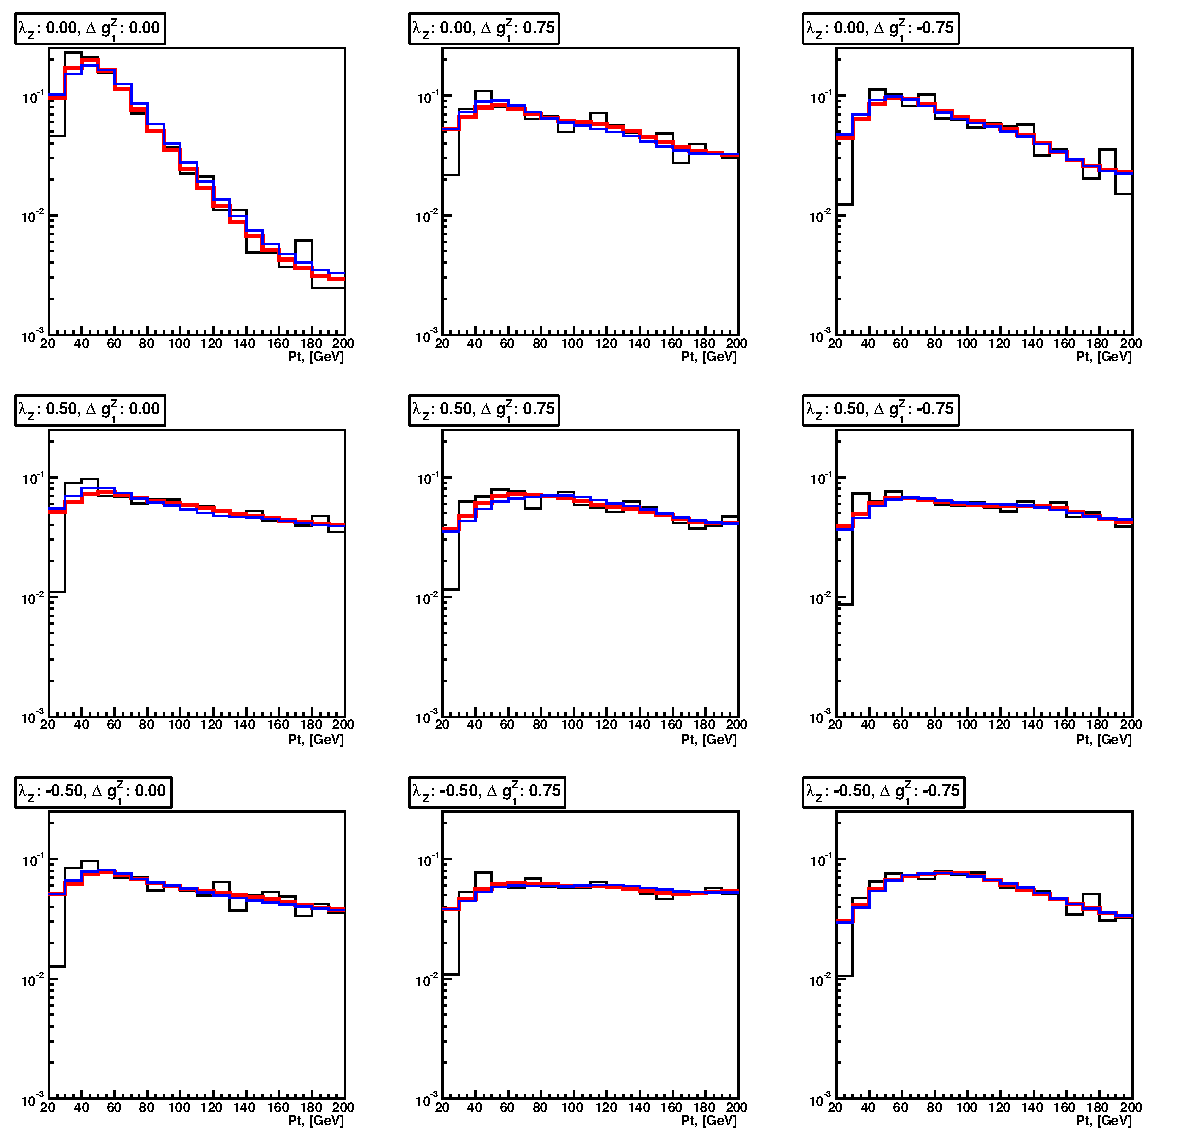
\includegraphics[width=1.0\textwidth]{figures/pdfs}
  }

  \caption[PDF parameterization] {Leading lepton \pt\ distributions
  for \ww\ events with and without aTGCs. The black points represent the
  true \pt\ distribution for Monte Carlo events that passed the final
  selection. The blue dots show the \pt\ distribution from the model used to
  parametrize the anomalous coupling effects across different values
  of the couplings.}
\label{fig:pdfs}
\end{figure}

Figure~\ref{fig:bkgpdfs} shows the leading lepton \pt\ PDFs
for background events. It is important to note that some of the major
backgrounds have harder leading lepton \pt\ distributions than Standard
Model $WW$, which may bias the result if not handled properly.

\begin{figure}[tp]
  \centerline{
    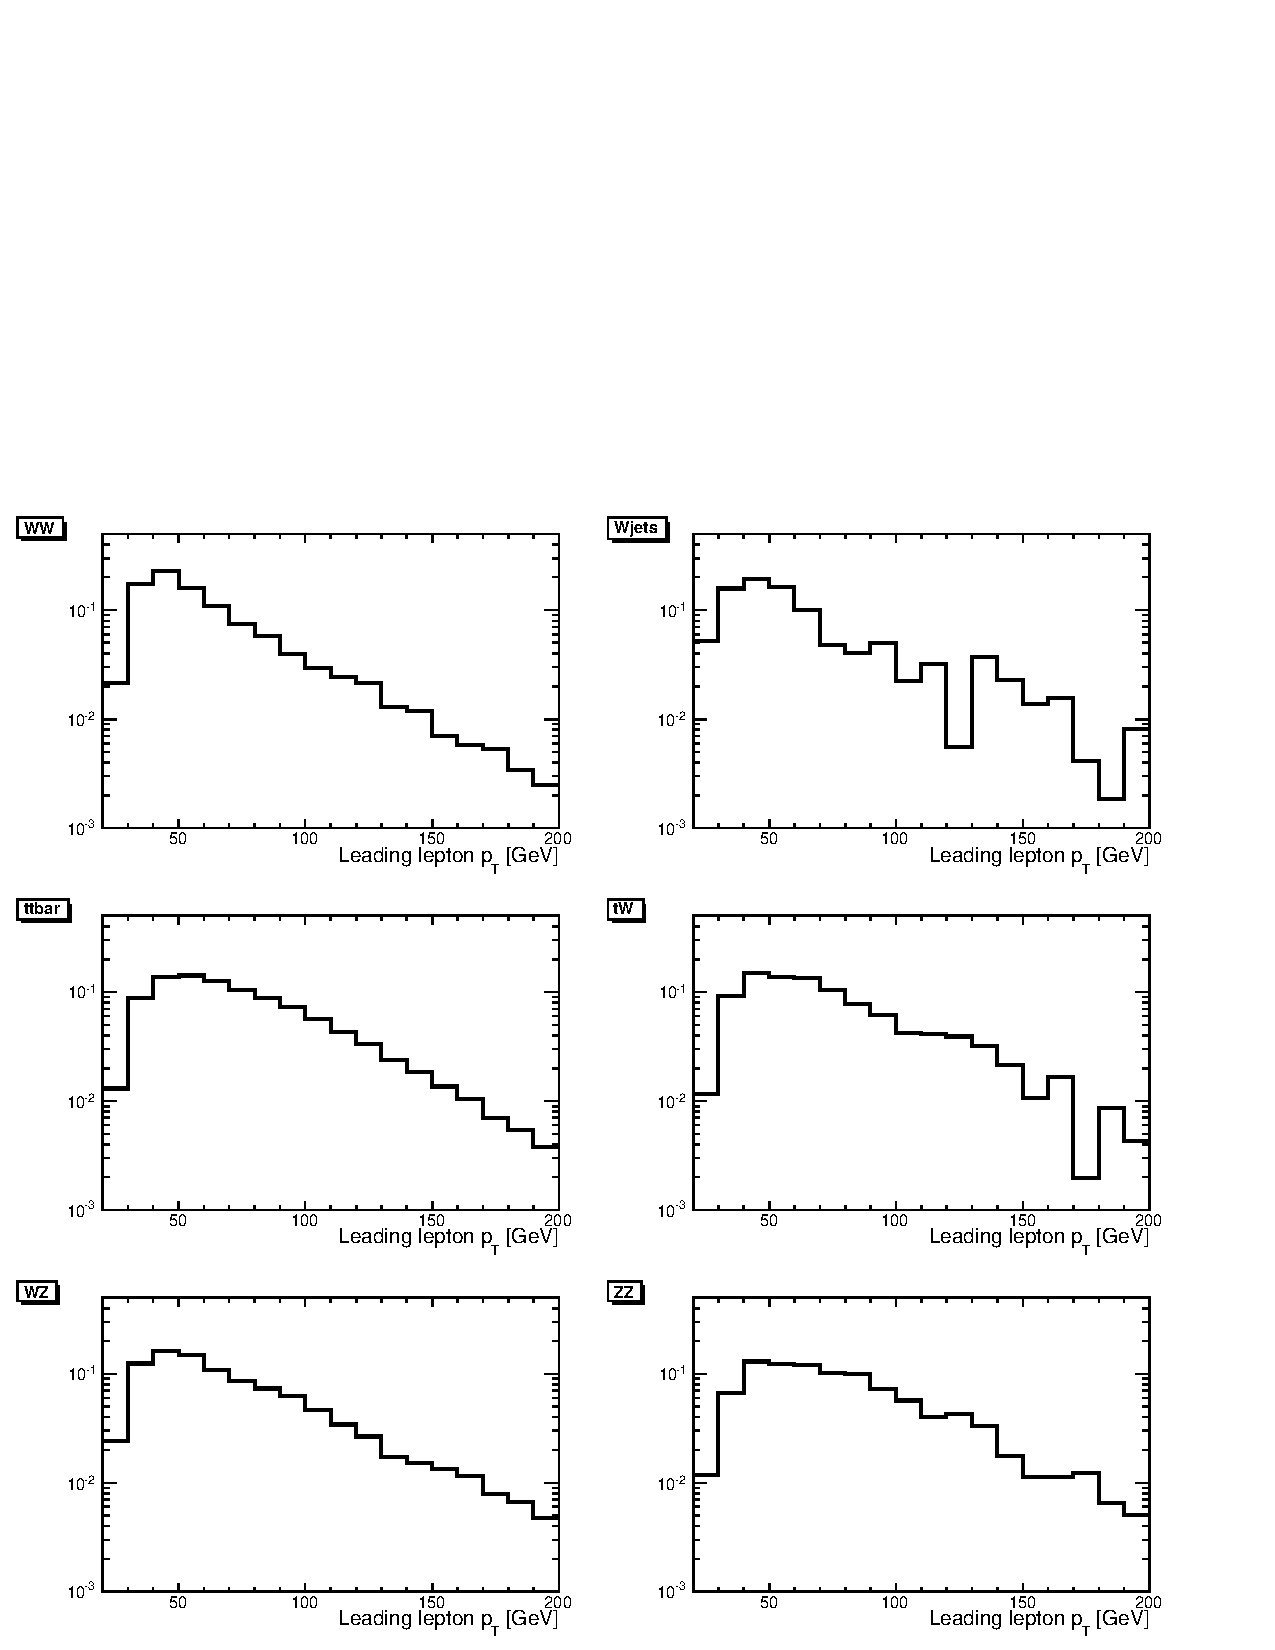
\includegraphics[width=0.7\textwidth]{figures/pdf_mc_all.pdf}
  }

  \caption[Background PDFs] {Leading lepton \pt\ PDFs for background
  events after full event selection.} \label{fig:bkgpdfs}
\end{figure}

\section{Closure tests}
   \label{sec:closure}
   The performance of the \zm\ method are evaluated in the following cases:
\begin{itemize}
\item on MC and on data;
\item inside and outside the Z peak;
\item at \WW\ level and after \mHi=120 \GeVcc\ selection.
\end{itemize}

The selection applied includes all \hww\ analysis cuts, except that, in order to increase the \dyll\ sample, 
the $\Delta\phi$(ll,jet1)$<$165$^\circ$ cut and the VBF selection in the 2-jet bin are not applied.
When considering  \mHi=120 \GeVcc\ selection, additional cuts are: dilepton mass $<$40 \GeVcc (not applied for tests under Z peak), 
$\Delta\phi$($l_1$,$l_2$)$<$115$^\circ$ and 70$<$$m_T$$<$120 \GeVcc.
In data, \dyll\ is always considered after \V\Z\ and opposire flavor subtraction.

Given that no information on the leptons can be extracted from the photon sample, the \zm\ method works only if no significant contribution to \met\ is 
due to lepton mismeasurement. 
This assumption can be tested looking at the observed number of events after the full \met\ cuts: 
we expect that the ratio of $\mu\mu$ to ee scales as the selection efficiency and is of the order of $\sim 1.7$.
However, this ratio may be subject to large fluctuations because the subtraction of \V\Z\ and opposite flavor events 
can be large and because \dyll\ samples (both data and MC) have limited statistics after full selection.

Tables~\ref{tab:mc_closure_ww_zv}-\ref{tab:data_closure_120_zv} summarize the result of the performed closure tests.
We define ``Observed'' as the \dyll\ yield in the pass region; ``Predicted'' as the \dyll\ yield extrapolating from the fail region using the \zm\ method;
``Bias'' as (Predicted-Observed)/Observed.
These results suggest a conservative systematic error of 40\% per channel (ee and $\mu\mu$).

%%%%%
\begin{table}[!ht]
\begin{center}
\begin{tabular} {|c|ccc|}
\hline
$N_{jets}$  & Observed & Predicted & Bias (\%) \\
\hline 
\hline
\multicolumn{4}{|c|}{di-muon final state} \\
\hline
0 & 10.0$\pm$2.9 &  7.8$\pm$2.0 & -22$\pm$36 \\
1 & 42.3$\pm$3.8 & 41.6$\pm$1.4 &  -2$\pm$11 \\
2 & 20.7$\pm$3.2 & 19.1$\pm$0.9 &  -8$\pm$16 \\
\hline 
\hline
\multicolumn{4}{|c|}{di-electron final state} \\
\hline
0 &  6.7$\pm$2.4 &  4.3$\pm$1.2 & -36$\pm$40 \\
1 & 28.9$\pm$3.8 & 23.9$\pm$0.9 & -17$\pm$13 \\
2 &  9.0$\pm$1.2 & 10.8$\pm$0.6 &  21$\pm$15 \\
\hline 
\end{tabular}
\caption{Closure test on MC at WW level with Z veto.}
\label{tab:mc_closure_ww_zv}
\end{center}
\end{table}
%%%%%



%%%%%
\begin{table}[!ht]
\begin{center}
\begin{tabular} {|c|ccc|}
\hline
$N_{jets}$  & Observed & Predicted & Bias (\%) \\
\hline 
\hline
\multicolumn{4}{|c|}{di-muon final state} \\
\hline
0 &  6.0$\pm$2.4 &  4.5$\pm$1.3 & -24$\pm$46 \\
1 & 14.5$\pm$3.5 & 12.7$\pm$1.0 & -13$\pm$25 \\
2 &  3.9$\pm$2.3 &  4.0$\pm$0.4 &   1$\pm$59 \\
\hline 
\hline
\multicolumn{4}{|c|}{di-electron final state} \\
\hline
0 & 4.3$\pm$2.3 & 2.3$\pm$0.9 & -47$\pm$52 \\
1 & 5.9$\pm$2.4 & 6.6$\pm$0.6 &  12$\pm$47 \\
2 & 1.0$\pm$0.5 & 1.7$\pm$0.2 &  67$\pm$55 \\
\hline 
\end{tabular}
\caption{Closure test on MC after \mHi=120 \GeVcc\ selection with Z veto.}
\label{tab:mc_closure_120_zv}
\end{center}
\end{table}
%%%%%

%%%%%
\begin{table}[!ht]
\begin{center}
\begin{tabular} {|c|ccc|}
\hline
$N_{jets}$  & Observed & Predicted & Bias (\%) \\
\hline 
\hline
\multicolumn{4}{|c|}{di-muon final state} \\
\hline
0 & 117$\pm$16 & 183$\pm$36 & 56$\pm$34 \\
1 & 977$\pm$33 & 963$\pm$53 & -1$\pm$6  \\
2 & 537$\pm$24 & 582$\pm$28 &  8$\pm$7 \\
\hline 
\hline
\multicolumn{4}{|c|}{di-electron final state} \\
\hline
0 &  95$\pm$13 & 106$\pm$22 &  12$\pm$27 \\
1 & 717$\pm$28 & 623$\pm$33 & -13$\pm$6  \\
2 & 468$\pm$22 & 384$\pm$18 & -18$\pm$6  \\
\hline 
\end{tabular}
\caption{Closure test on data at WW level in Z peak.}
\label{tab:data_closure_ww_zp}
\end{center}
\end{table}
%%%%%

%%%%%
\begin{table}[!ht]
\begin{center}
\begin{tabular} {|c|ccc|}
\hline
$N_{jets}$  & Observed & Predicted & Bias (\%) \\
\hline 
\hline
\multicolumn{4}{|c|}{di-muon final state} \\
\hline
0 &  44$\pm$25 &  47$\pm$10 &  7$\pm$61 \\
1 & 200$\pm$23 & 211$\pm$17 &  5$\pm$14 \\
2 & 128$\pm$18 & 123$\pm$10 & -4$\pm$16 \\
\hline 
\hline
\multicolumn{4}{|c|}{di-electron final state} \\
\hline
0 &  40$\pm$18 &  30$\pm$7 & -26$\pm$49 \\
1 & 168$\pm$18 & 118$\pm$8 & -29$\pm$12  \\
2 &  88$\pm$14 &  76$\pm$6 & -14$\pm$17 \\
\hline 
\end{tabular}
\caption{Closure test on data at WW level with Z veto.}
\label{tab:data_closure_ww_zv}
\end{center}
\end{table}
%%%%%

%%%%%
\begin{table}[!ht]
\begin{center}
\begin{tabular} {|c|ccc|}
\hline
$N_{jets}$  & Observed & Predicted & Bias (\%) \\
\hline 
\hline
\multicolumn{4}{|c|}{di-muon final state} \\
\hline
0 &  68$\pm$9  &  61$\pm$14 & -10$\pm$24 \\
1 & 250$\pm$16 & 298$\pm$32 &  19$\pm$14 \\
2 &  97$\pm$10 & 143$\pm$19 &  47$\pm$22 \\
\hline 
\hline
\multicolumn{4}{|c|}{di-electron final state} \\
\hline
0 &  42$\pm$7  &  35$\pm$8  & -17$\pm$26 \\
1 & 168$\pm$13 & 190$\pm$20 &  13$\pm$14 \\
2 &  95$\pm$10 &  91$\pm$10 &  -4$\pm$15 \\
\hline 
\end{tabular}
\caption{Closure test on data after \mHi=120 \GeVcc\ selection in Z peak.}
\label{tab:data_closure_120_zp}
\end{center}
\end{table}
%%%%%

%%%%%
\begin{table}[!ht]
\begin{center}
\begin{tabular} {|c|ccc|}
\hline
$N_{jets}$  & Observed & Predicted & Bias (\%) \\
\hline 
\hline
\multicolumn{4}{|c|}{di-muon final state} \\
\hline
0 & 25$\pm$10 & 22$\pm$5  & -13$\pm$46 \\
1 & 62$\pm$9  & 72$\pm$13 &  17$\pm$25 \\
2 & 42$\pm$8  & 35$\pm$8  & -18$\pm$26 \\
\hline 
\hline
\multicolumn{4}{|c|}{di-electron final state} \\
\hline
0 &  0$\pm$6 &  7$\pm$2 &    nan    \\
1 & 30$\pm$6 & 32$\pm$5 &  7$\pm$28 \\
2 & 14$\pm$5 & 17$\pm$4 & 26$\pm$44 \\
\hline 
\end{tabular}
\caption{Closure test on data after \mHi=120 \GeVcc\ selection with Z veto.}
\label{tab:data_closure_120_zv}
\end{center}
\end{table}
%%%%%

\clearpage

\section{Comparison with \routin~ method}
   \label{sec:comparison}
   placeholder

\section{Conclusion}
   We presented a study of the anomalous triple gauge couplings in \wwll\
decays reconstructed from Run2010A and Run2010B data collected at 7
TeV center of mass energy. With around 10 signal and 3 background
events in the final dataset we performed unbinned maximum likelihood
fits for the leading lepton \pt\ distribution and the total number of
signal events. The results that we get are consistent with the
Standard Model. The exclusion limits are in general comparable to those
of the Tevatron. In order to achieve the
current world average limits on anomalous couplings a dataset of the
order of 5~\ifb is necessary.

\clearpage
\clearpage

\vspace*{-0.2cm}
\thebibliography{12}

\bibitem{pdg}
 K. Nakamura et al. (Particle Data Group), "Review of particle physics", J. Phys.G37 , 2010.

\bibitem{Higgs1}
F. Englert and R. Brout, "Broken symmetries and the masses of gauge bosons", Phys. Rev. Lett. 13,  1964.

\bibitem{Higgs2}
P. W. Higgs, "Broken symmetry and the mass of gauge vector mesons", Phys. Rev. Lett. 13, 1964.

\bibitem{Higgs3}
Guralnik, G.S. and Hagen, C.R. and Kibble, T.W.B., "Global Conservation Laws and Massless Particles", 
Phys.Rev.Lett. 13, 1964.

\bibitem{dittmar}
M.~Dittmar and H.~K.~Dreiner, Phys.\ Rev.\  D {\bf 55} (1997) 167".

\bibitem{HWW2010}
CMS Collaboration, "Measurement of WW Production and Search for the Higgs Boson in 
pp Collisions at $\sqrt{s}$ = 7 TeV", arXiv:1102.5429

\bibitem{HWW2011AN}
L.~Bauerdick et al, "A Higgs Boson Search in the Fully Leptonic $W^+W^-$ Final State", CMS AN-2011/155

\bibitem{VBTFCrossSectionNote}
J. Alcaraz Maestre, \textit{et al.}, "Updated Measurements of Inclusive W and Z Cross Sections 
at $\sqrt{s}=7$ TeV", CMS AN-2010/264.

\bibitem{ggWWError}
F.~ Stoeckli, "http://indico.cern.ch/getFile.py/access?contribId=0\&resId=1\&materialId=slides\&confId=49009", 
EWK Diboson meeting of March 12 2009.

\bibitem{json}
{\small
/afs/cern.ch/cms/CAF/CMSCOMM/COMM\_DQM/certification/Collisions11/7TeV/Prompt/Cert\_160404-163869\_7TeV\_PromptReco\_Collisions11\_JSON.txt
}

\bibitem{ElIso}
A. Vartak, M. LeBourgeois, V. Sharma, "Lepton Isolation in the CMS Tracker, ECAL and HCAL", CMS AN-2010/106.

\bibitem{PVDA}
W. Erdmann, M. LeBourgeois, B. Mangano, 
https://indico.cern.ch/getFile.py/access?contribId=5\&sessionId=3\&resId=1\&materialId=slides\&confId=127127, 
note in preparation.

\bibitem{NExpHits}
B. Mangano \textit{et al.}, "Improvement in Photon Conversion Rejection Performance Using 
Advanced Tracking Tools", AN-10-283.

\bibitem{fakeLeptonNote1}
S.~Xie, \textit{et al.}", "Study of Data-Driven Methods for Estimation of Fake Lepton Backgrounds", 
CMS AN-2009/120.

\bibitem{fakeLeptonNote2}
W.~Andrews, \textit{et al.}, "Fake Rates for dilepton Analyses", CMS AN-2010/257.

\bibitem{fakeLeptonBkgSpillage1}
 F. Golf, D. Evans, J. Mulmenstadt  \textit{et al.}, ``Expectations for observation of top quark pair production in the dilepton final state with the early CMS data'', CMS AN-2009/050.

\bibitem{dyestnote}
W. Andrews, et al., “A Method to Measure the Contribution of $\dyll$ to a di-lepton+ MET Selection”, CMS AN-2009/023 (2009).

\bibitem{jes}
CMS Collaboration, "Jet Energy Calibration with Photon+Jet Events", PAS JME-09-004.

\bibitem{jetpas}
CMS Collaboration, "Jet Performance in pp Collisions at $\sqrt{s}=7 \rm\ TeV$", PAS JME-10-003.

\bibitem{btag}
CMS collaboration, "Commissioning of b-jet identification with pp collisions at $\sqrt{s}=7~\TeV$, BTV-10-001.

\bibitem{antikt}
Cacciari, Matteo and Salam, Gavin P. and Soyez, Gregory, "The anti-$k_t$ jet clustering 
algorithm", JHEP 04,  2008.

\bibitem{ConversionNote}
W.~Andrews, \textit{et al.}, "Study of photon conversion rejection at CMS", CMS AN-2009/159.

\bibitem{tmva}
A. Hoecker, \textit{et al.}, "TMVA - Toolkit for Multivariate Data Analysis", arXiv:physics/0703039, 2007.

\bibitem{XS}
CMS Generator group, Standard Model Cross Sections for CMS at 7 TeV, 2010.

\bibitem{PDF4LHC}
PDF4LHC Working Group, 
{\tt http://www.hep.ucl.ac.uk/pdf4lhc/PDF4LHCrecom.pdf}

\bibitem{Nadolsky:2008zw}
Nadolsky, Pavel M. and others, "Implications of CTEQ global analysis for 
collider observables", Phys. Rev. D78 2008.

\bibitem{Martin:2009iq}
Martin, A. D. and Stirling, W. J. and Thorne, R. S. and Watt, G., "Parton 
distributions for the LHC, Eur. Phys. J. C63 2009.

\bibitem{Ball:2010de}
Ball, Richard D. and others, "A first unbiased global NLO determination 
of parton distributions and their uncertainties", arXiv 1002.4407.

\bibitem{bayesian}
A. O'Hagan and J.J. Forster, "Bayesian Inference", Kendall's Advanced Theory of Statistics, 
Arnold, London, 2B, 2004.

\bibitem{ref:tagprobe_mit_w}
G. Bauer {\it et. al.}, "Lepton ef?iencies for the inclusive W cross section measurement with 36.1pb$^{-1}$", AN2011/097

\bibitem{ref:tagprobe_snt_top}
W. Andrews {\it et. al.}, "Uncertainties on the Lepton Selection Efficiency for t$t\bar{t}$ Cross Section Analysis", AN2010/274

\bibitem{LHCHiggsCrossSectionWorkingGroup:2011ti}
LHC Higgs Cross Section Working Group, "Handbook of LHC Higgs Cross Sections: 
Inclusive Observables", CERN-2011-002, 2011.

\bibitem{PFMET} 
CMS Collaboration, ``CMS MET Performance in Events Containing Electroweak Bosons from pp Collisions at $\sqrt{s}=7$ TeV'', CMS PAS JME-2010-005 (2010)


\bibitem{trkMET} 
Marco Zanetti, ``MET with PU in $\hww\to2\ell$'', https://indico.cern.ch/conferenceDisplay.py?confId=131580
Benjamin Hooberman, ``MET with PU in MC and First 2011 Data'', https://indico.cern.ch/contributionDisplay.py?contribId=5\&confId=132579. 


\bibitem{lands}
Mingshui Chen and Andrey Korytov, https://mschen.web.cern.ch/mschen/lands/

\bibitem{MCFMHiggsProduction}
J. Campbell, R.K. Ellis, G. Zanderighi, ``Next-to-Leading order Higgs + 2 jet production via gluon fusion.'', JHEP 0610:028 (2006), hep-ph/0608194

\bibitem{MCFMVVProduction}
J. Campbell, R.K. Ellis, C. Williams, ``Vector boson pair production at the LHC.'', arxiv:hep-ph/1105.0020.

\bibitem{MITHggNote} 
G. Bauer et al., ``Higgs Search in the pp $\rightarrow$ H $\rightarrow$ $\gamma\gamma$ channel at $\sqrt{s}=7$ TeV'', CMS AN-2011/168. 


\end{document}
